\documentclass{article}

% Language setting
% Replace `english' with e.g. `spanish' to change the document language
\usepackage[english]{babel}
\usepackage{listings}
\usepackage{xcolor}

% Set page size and margins
% Replace `letterpaper' with `a4paper' for UK/EU standard size
\usepackage[letterpaper,top=2cm,bottom=2cm,left=3cm,right=3cm,marginparwidth=1.75cm]{geometry}

% Useful packages
\usepackage{amsmath}
\usepackage{graphicx}
\usepackage[colorlinks=true, allcolors=blue]{hyperref}

\lstset{
    language=C++,
    backgroundcolor=\color{black!5}, 
    basicstyle=\footnotesize\ttfamily,
    keywordstyle=\color{magenta},
    commentstyle=\color{green!60!black},
    numbers=left,
    breaklines=true,
    frame=single
}
% \lstset{
%     language=binary,
%     basicstyle=\ttfamily\small, % Monospace font and size
%     breaklines=true,            % Allows the line to wrap
%     columns=fixed,              % Ensures characters align
%     tabsize=4,                  % Define tab size (if tabs are used)
%     rulecolor=\color{black},    % Color of the frame (if used)
%     frame=single               % Uncomment to add a frame around the listing
% }
\title{A Compile-Time and Memory-Efficient Approach to SunSpec Models with Google's  FlatBuffers in Embedded Systems and Direct Modbus Register Mapping}
\author{Busoye Tolulope Matthew}


\begin{document}
\maketitle

\section{Overview}
\label{sec:overview}
The SunSpec Alliance defines standard information models for the interoperability of distributed energy resources, typically represented through Modbus register maps on embedded systems. Traditional approaches to implementing SunSpec rely on static C structures, JSON, or XML-based model definitions. However, these methods present challenges: XML and JSON parsing are memory-intensive and computationally inefficient for small microcontrollers, while static structures lack flexibility.
This paper presents a method for representing SunSpec model definitions using FlatBuffers, a binary serialization format designed for zero-copy access. Model definitions are compiled into a compact binary format that can be included in embedded firmware, eliminating runtime parsing costs and avoiding unnecessary RAM usage. Definitions may also be stored externally in read-only memory or on removable storage (e.g., SD card) and loaded on demand. Furthermore, the Modbus register layout is directly mapped onto contiguous memory buffers, ensuring that SunSpec point values can be read or written with statically predefined memory allocation.
The proposed library enables developers to include only the SunSpec models required for their device at compile time, thereby minimizing code size. By leveraging FlatBuffers and contiguous Modbus memory layouts, this approach provides an efficient and scalable method for building SunSpec-compliant devices and gateways suitable for resource-constrained embedded systems.

\section{Introduction}
\label{sec:introduction}

\subsection{Sunspec Alliance}
The SunSpec Alliance is an industry-standard body that provides information models for Distributed Energy Resources (DERs), such as solar inverters, battery storage systems, and meters. These models define a consistent mapping of across same device from different manufacturers. By standardizing the communication layer—typically over Modbus—SunSpec ensures interoperability between hardware from different vendors and monitoring software. However, as the complexity of DERs increases (e.g., the transition from IEEE 1547-2018 to advanced grid-support functions), the number of required SunSpec models grows, placing a significant burden on the firmware of the local controllers. 

SunSpec Device Information Models provide a simple, standardized mechanism for specifying data sets supported by a device.
Device Information Model definitions represent collections of device data points. Figure \ref{fig:model_def_image} shows the structural relationship of the different elements of the definitions.
Device Information Models are defined using the following definition elements:
\begin{itemize}
\item \textbf{Models} are used to hold all elements, and it serves as the logical container for all related data points.
    \item \textbf{Point Group} or Groups are used to hold logically related point together. It could either be a top level group, a repeated set os points or a set of point with synchronous operational requirements.
    \item \textbf{Points} hold the device models data.
    \item \textbf{Symbols} define the set of valid values for the point and provide identifiers that can be used to represent the value.
3.1.5
    \item \textbf{Comment} is used to document the element definition.
\end{itemize}
\begin{figure}
    \centering
    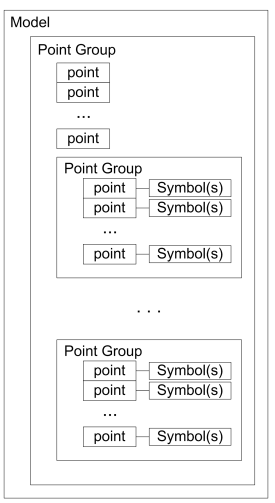
\includegraphics[width=0.5\linewidth]{sunspec_model_definition.png}
    \caption{Device Information Model Structure}
    \label{fig:model_def_image}
\end{figure}

\subsection{Google's  Flatbuffers}
FlatBuffers is an open-source, cross-platform serialization library originally developed for high-performance applications like game development. Its defining feature is zero-copy deserialization. Unlike most serialization formats. A FlatBuffer is a binary buffer containing nested objects (structs, tables, vectors,..) organized using offsets so that the data can be traversed in-place just like any pointer-based data structure.

The FlatBuffer compiler (flatc) generates C++ or C headers that allow the application to treat the binary data as if it were a native memory-mapped structure. This makes it uniquely suited for systems where CPU cycles and heap memory are at a premium.

\subsection{Serialization Frameworks and their Issues in Embedded Systems}
While various serialization frameworks exist, most fail to meet the rigorous constraints of low-power microcontrollers (e.g., ARM Cortex-M series). The primary issues include:
\begin{itemize}
\item Computational Overhead: XML and JSON are text-based, requiring heavy string manipulation and lexical analysis. This consumes significant CPU cycles and battery power.

\item Memory Overhead and Fragmentation: Common libraries for Protobuf or JSON often rely on dynamic memory allocation (malloc/free) to build a Document Object Model (DOM) in RAM. In embedded systems, this leads to heap fragmentation and potential runtime crashes.

\item Flash Footprint: Generic parsers often have large code footprints. For a device with only 256KB of Flash, a full XML parser is often too large to be viable.

\end{itemize}

\section{Sunspec Flatbuffers Implementation}
The source code of the library can be found \url{https://github.com/thew0205/sunspec_flatbuffers}.
\subsection{Sunspec Schema Definition and C++ Code Generation}
The SunSpec Device Information Model Specification document defines the Device Information Model Definition which includes three major elements which are the model, group, and point. The other two, symbols and comments will not be included in the implementation as symbols define name, value pairs for constant values or enumerations which just bloat the resulting binary and these names are rarely used in embedded systems.

The implementation of the definition in flatbuffers schema can be seen in Listing \ref{lst:schema}. As can be seen, there is a one to one mapping of the definition to the flatbuffers schema.

 \begin{lstlisting}[language=C++, caption={Sunspec Flatbuffers Schema Definition}, label={lst:schema}]
 enum SunspecPointAccessType :uint8
{
    kR,  /**< Only access Read supported */
    kRW, /**< Read and Write access supported */
}

/**
 * @brief Enumeration of SunspecPoint mandatory types.
 */
enum SunspecPointMandatoryType: uint8
{
    kM, /**< Point must be implemented */
    kO, /**< Point can be omitted */
}

union SunspecPointData
{
    // kUndefinedType = 0, /**< Undefined type */
    kSint16,             /**< Signed 16-bit integer */
    kSint32,             /**< Signed 32-bit integer */
    kSint64,             /**< Signed 64-bit integer */
    kRaw16,             /**< 16-bit raw value */
    kUint16,            /**< Unsigned 16-bit integer */
    kUint32,            /**< Unsigned 32-bit integer */
    kUint64,            /**< Unsigned 64-bit integer */
    kAcc16,             /**< Unsigned 16-bit accumulator(deprecated, in favor of uint16) */
    KAcc32,             /**< Unsigned 32-bit accumulator (deprecated in favor of uint32) */
    kAcc64,             /**< Unsigned 64-bit accumulator (deprecated in favor of uint64) */
    kBitField16,        /**< 16-bit bitfield */
    kBitField32,        /**< 32-bit bitfield */
    kBitField64,        /**< 64-bit bitfield */
    kEnum16,            /**< 16-bit enumeration */
    kEnum32,            /**< 32-bit enumeration */
    kFloat32,           /**< 32-bit floating-point */
    kFloat64,           /**< 64-bit floating-point */
    kString,            /**< String (UTF-8 encoded) */
    kSunsSf,            /**< Scale factor Signed power of 10 multiplier (+) or divider (-) */
    kPad16,               /**< 16-bit pad used for alignment */
    kIpAddr,            /**< IP Address as an unsigned 32-bit. */
    kIpv6Addr,          /**< 16-byte IP V6 address */
    kEui48,             /**< 48-bit MAC address */
}

table SunspecPointDef{
    id : string;
    data: SunspecPointData;
    // This is need because it can be specified as a constant in the model definition or in another point.
    count:uint16= 1;
    count_point_id : string;
    size: uint16;
    sf : int16;
    sf_id : string;
    units : string;
    access:SunspecPointAccessType = kR;
    mandatory:SunspecPointMandatoryType = kO;
    label : string;
}

enum SunspecGroupType:uint8
{
    kGroup,
    kSync,
}

table SunspecGroupPointDef{
    id: string;
    type:SunspecGroupType = kGroup;
    count:uint16 = 1;
    count_point_id:string;
    points: [SunspecPointDef];
    groups: [SunspecGroupPointDef];
    label:string;
}

table SunspecModelDef{
    id: SunspecModelList = 0xFFFF;
    group:SunspecGroupPointDef;
}

root_type SunspecModelDef;
\end{lstlisting}

The schema is then passed the flatbuffers compiler flatc to generate the equivalent c++ code which is then use to parse the generated binary representing the sunspec model definition.
Snippect from the generated code is shown in Listing \ref{lst:generated_code}, the code shown is the generated code to access (deserialization is a minomer in flatbuffers as no serialization is done) the data of the SunspecModelDef, and also to access the Root SunspecModelDef from the result binary buffer. We only care about the de-serialization code as the serialization will be done by the flatbuffers compiler.

\begin{lstlisting}[language=C++, caption={Sunspec Flatbuffers Schema Definition}, label={lst:generated_code}]
struct SunspecModelDef FLATBUFFERS_FINAL_CLASS : private ::flatbuffers::Table {
  typedef SunspecModelDefBuilder Builder;
  enum FlatBuffersVTableOffset FLATBUFFERS_VTABLE_UNDERLYING_TYPE {
    VT_ID = 4,
    VT_GROUP = 6
  };
  SunspecModelList id() const {
    return static_cast<SunspecModelList>(GetField<uint16_t>(VT_ID, 0));
  }
  const SunspecGroupPointDef *group() const {
    return GetPointer<const SunspecGroupPointDef *>(VT_GROUP);
  }
  template <bool B = false>
  bool Verify(::flatbuffers::VerifierTemplate<B> &verifier) const {
    return VerifyTableStart(verifier) &&
           VerifyField<uint16_t>(verifier, VT_ID, 2) &&
           VerifyOffset(verifier, VT_GROUP) &&
           verifier.VerifyTable(group()) &&
           verifier.EndTable();
  }
};

inline const SunspecModelDef *GetSunspecModelDef(const void *buf) {
  return ::flatbuffers::GetRoot<SunspecModelDef>(buf);
}
\end{lstlisting}

\subsection{Generating and Serializing Sunspec Data}
The flatbuffers compiler apart from generating code from the schema to different language, can also generate flatbuffers binary representation of data from json documents. Though the sunspec aliance group provide a json format of model definition, this specification has some errors and incohenrence, also a few modification had to be made for the format to align with the flabuffers schema defined. Some of the mistakes observed with some points had count field has 0(which represent the count is held by another point) rather than the being a constant value or the id of the point with the count, which has to be explored and set manually.

The new generated json files were passed to the flatbuffers compile along with the schema to genrate the raw binary.

\begin{lstlisting}[caption={Generated Binary for Model 1}, label={lst:mode11_bin}]
00000000: 0c00 0000 0800 0e00 0600 0800 0800 0000  ................
00000010: 0000 0100 1800 0000 0000 1200 1400 0400  ................
00000020: 0000 0000 0000 0800 0c00 1000 1200 0000  ................
00000030: 2402 0000 1c00 0000 1400 0000 0400 0000  $...............
00000040: 0600 0000 436f 6d6d 6f6e 0000 0000 0000  ....Common......
00000050: 0900 0000 d401 0000 8801 0000 3c01 0000  ............<...
00000060: 1401 0000 ec00 0000 a800 0000 7800 0000  ............x...
00000070: 4800 0000 1400 0000 1000 0c00 0800 0500  H...............
00000080: 0000 0000 0000 0600 1000 0000 0014 0100  ................
00000090: 0400 0000 0300 0000 5061 6400 1c00 1000  ........Pad.....
000000a0: 0800 0400 0000 0000 0000 0600 0000 0000  ................
000000b0: 0000 0500 0000 0c00 1c00 0000 0501 0100  ................
000000c0: 1c00 0000 0400 0000 0e00 0000 4465 7669  ............Devi
000000d0: 6365 2041 6464 7265 7373 0000 0200 0000  ce Address......
000000e0: 4441 0000 20ff ffff 1200 1000 1c00 0000  DA.. ...........
000000f0: 0400 0000 0d00 0000 5365 7269 616c 204e  ........Serial N
00000100: 756d 6265 7200 0000 0200 0000 534e 0000  umber.......SN..
00000110: dcff ffff 0012 0800 1400 0000 0400 0000  ................
00000120: 0700 0000 5665 7273 696f 6e00 0200 0000  ....Version.....
00000130: 5672 0000 1c00 1000 0800 0500 0000 0000  Vr..............
00000140: 0000 0600 0000 0000 0000 0000 0000 0c00  ................
00000150: 1c00 0000 0012 0800 1400 0000 0400 0000  ................
00000160: 0700 0000 4f70 7469 6f6e 7300 0300 0000  ....Options.....
00000170: 4f70 7400 b0ff ffff 1200 1000 1400 0000  Opt.............
00000180: 0400 0000 0500 0000 4d6f 6465 6c00 0000  ........Model...
00000190: 0200 0000 4d64 0000 d4ff ffff 1200 1000  ....Md..........
000001a0: 1c00 0000 0400 0000 0c00 0000 4d61 6e75  ............Manu
000001b0: 6661 6374 7572 6572 0000 0000 0200 0000  facturer........
000001c0: 4d6e 0000 1c00 1000 0800 0400 0000 0000  Mn..............
000001d0: 0000 0600 0000 0000 0000 0000 0500 0c00  ................
000001e0: 1c00 0000 0500 0100 1c00 0000 0400 0000  ................
000001f0: 0c00 0000 4d6f 6465 6c20 4c65 6e67 7468  ....Model Length
00000200: 0000 0000 0100 0000 4c00 0000 1c00 1400  ........L.......
00000210: 0800 0400 0c00 0000 0000 0600 0000 0000  ................
00000220: 0000 0000 0500 1000 1c00 0000 0500 0100  ................
00000230: 1c00 0000 1600 0000 0400 0000 0800 0000  ................
00000240: 4d6f 6465 6c20 4944 0000 0100 0200 0000  Model ID........
00000250: 4944 0000 0600 0000 636f 6d6d 6f6e 0000  ID......common..
\end{lstlisting}
Listing \ref{lst:mode11_bin} shows the output for flatbuffers inary generated for model 1. The resulting binary file is 608 bytes without any compression as compared to the original json file of 3381 bytes.
\subsection{Integrating with C++ code }
\label{sec:integrating}
Listing \ref{lst:generated_code_group_point} show the access the sunspec model definition in the flatbuffers binary to initialized a sunspec group point.

The def\_ holds a reference to the sunspec group definition which is then accessed to get the points, which is vector of refence of sunspec point in the flatbuffers binary. The point definition has a count attribute that defines how many time the point is repeated: if the count in 0, that means the count is not fixed and it variable count is define in another point which name in the attribute count\_point\_id in the top level point. In the instanciation of each point, a reference to an inplace memory buffer is passed to it, these buffer has been preallocated and is guarranted the size specified of the point.

\begin{lstlisting}[language=C++, caption={Using the generated code and binary to actualize a sunspec GroupPoint}, label={lst:generated_code_group_point}]

void SunspecGroupReader::initPoints()
{
    // NOTE The toplevel point always have fixed count
    registerLength_ = 0;
    points_.clear();
    groups_.clear();

    vector<size_t> pointCounts;
    vector<const SunspecPointDef *> pointDefs;
    size_t totalPointCount = 0;

    for (const auto &pointDef : *def_.points())
    {
        uint16_t count = pointDef->count();
        if (0 == count)
        {
            // NOTE Count is always in the top levelgroup
            // NOTE All toplevel points have fixed count
            assert(!isTopLevelGroupPoint());

            SunspecPointReader *countPoint = getModel()->getPoint(FlatbufferStringToString(pointDef->count_point_id()));

            count = countPoint == nullptr ? 0 : countPoint->valueAsUint16();
            count = (count == kUint16UnimplementedValue) ? 0 : count;
        }

        totalPointCount += count;
        pointCounts.push_back(count);
        pointDefs.push_back(pointDef);
    }
    assert(pointCounts.size() == pointDefs.size() /*, "Internal error: pointCounts and pointDefs size mismatch"*/);

    points_.reserve(totalPointCount);
    for (size_t i = 0; i < pointCounts.size(); i++)
    {

        const auto pointDef = pointDefs[i];
        const auto count = pointCounts[i];
        if (count == 0)
        {
            continue;
        }

        for (size_t i = 0; i < count; i++)
        {
            points_.emplace_back(*pointDef, &modbusBuffer_[registerLength_], *this);
            registerLength_ += pointDef->size();
        }
    }
}
\end{lstlisting}

Listing \ref{lst:modbus_code} shows a sample of the code that extract the specific type from the modbus buffer that holds the appropriate value. The functions correct the modbus endianness to the correct endianness. 
\begin{lstlisting}[language=C++, caption={Access the point value from the inplace modbus buffer}, label={lst:modbus_code}]
nline uint32_t modbusRegisterFormatToUint32(const uint16_t *buffer)
{
    return ((static_cast<uint32_t>(buffer[0])) << 1 * 16) | ((static_cast<uint32_t>(buffer[1])));
}

inline double modbusRegisterFormatToDouble(const uint16_t *buffer)
{
    const uint64_t combined = modbusRegisterFormatToUint64(buffer);
    return *reinterpret_cast<const double *>(&combined);
}

inline const std::string modbusRegisterFormatToString(const uint16_t *buffer, const uint16_t bufferSize)
{
    char charBuffer[bufferSize * 2];
    for (size_t i = 0; i < bufferSize; i++)
    {
        charBuffer[i * 2] = (buffer[i] >> 8) & 0x00FF;
        charBuffer[i * 2 + 1] = buffer[i] & 0x00FF;
    }
    charBuffer[bufferSize * 2 - 1] = '\0';

    return std::string{charBuffer};
}

string SunspecPointReader::getValueAsString() const
{
    string ret;

    switch (def_.data_type())
    {

    case SunspecPointData_kSint16:
        ret += to_string(modbusRegisterFormatToSint16(modbusBuffer_));
        break;
    case SunspecPointData_kSunsSf:
        ret += to_string(modbusRegisterFormatToSunsSf(modbusBuffer_));
        break;

    case SunspecPointData_kUint16:
    case SunspecPointData_kPad16:
    case SunspecPointData_kBitfield16:
    case SunspecPointData_kAcc16:
    case SunspecPointData_kEnum16:
    case SunspecPointData_kRaw16:
        ret += to_string(modbusRegisterFormatToUint16(modbusBuffer_));
        break;

    case SunspecPointData_kSint32:
        ret += to_string(modbusRegisterFormatToSint32(modbusBuffer_));
        break;
    case SunspecPointData_kUint32:
    case SunspecPointData_kAcc32:
    case SunspecPointData_kBitfield32:
    case SunspecPointData_kEnum32:
        ret += to_string(modbusRegisterFormatToUint64(modbusBuffer_));
        break;

    case SunspecPointData_kSint64:
        ret += to_string(modbusRegisterFormatToSint64(modbusBuffer_));
        break;

    case SunspecPointData_kUint64:
    case SunspecPointData_kAcc64:
    case SunspecPointData_kBitfield64:
        ret += to_string(modbusRegisterFormatToUint64(modbusBuffer_));
        break;

    case SunspecPointData_kFloat32:
        ret += to_string(modbusRegisterFormatToFloat(modbusBuffer_));
        break;

    case SunspecPointData_kFloat64:
        ret += to_string(modbusRegisterFormatToDouble(modbusBuffer_));
        break;

    case SunspecPointData_kStringx:
        ret += modbusRegisterFormatToString(modbusBuffer_, def_.size());
        break;
    case SunspecPointData_kIpAddr:
    case SunspecPointData_kIpv6Addr:
    case SunspecPointData_kEui48:
    case SunspecPointData_NONE:
    default:

        break;
    }

    return ret;
}
\end{lstlisting}

\section{Empirical Evaluation of Model-Definition Backends}
\label{sec:evaluation}

{\sloppy This section compares three interchangeable model-definition backends on the class of hardware the library targets. All three implement the identical \texttt{SunspecModelDef}/\allowbreak\texttt{SunspecGroupDef}/\allowbreak\texttt{SunspecPointDef} accessor surface described in Section~\ref{sec:integrating}:\par}

\begin{itemize}
    \item \textbf{flatbuffers} -- the approach proposed in this paper: each model is a pre-compiled FlatBuffers binary stored in flash and read in place through the generated zero-copy accessors.
    \item \textbf{c\_define} -- each model is written as native C++ constructor calls; when the model list is initialised, they build a tree of \texttt{std::vector}, \texttt{std::variant} and \texttt{std::string\_view} objects.
    \item \textbf{json} -- each model is stored in flash as JSON text and tokenised on demand with the jsmn tokeniser.
\end{itemize}

The backend is selected by a single compile-time switch, and everything above it -- including the benchmark code itself -- compiles unchanged against all three.

\subsection{Experimental Setup}
All measurements were taken on a Raspberry Pi Pico2 board (RP2350, Arm Cortex-M33 at 150\,MHz, 512\,KB SRAM, 4\,MB QSPI flash). Firmware was built with the Raspberry Pi Pico SDK 2.2.0 and \texttt{arm-none-eabi-gcc} 14.2.1 for the \texttt{rp2350-arm-s} platform in the \texttt{Release} configuration (\texttt{-O3 -g}).

\subsection{Benchmark Variants}
For each backend, four firmware images were built. They differ in the \texttt{walk()} function each links in from \path{experiment/common/}:

\begin{itemize}
    \item \textbf{noop} -- does not call the SunSpec library, and is built with a copy of the harness that makes no library calls either (\texttt{harness\_main\_noop.cpp}), so it links nothing from the library. It is the baseline for flash, RAM, heap and time.
    \item \textbf{load\_only} -- calls \texttt{initializeAllModels()}. This links the complete backend with all 112 models; once the model list exists, the call only checks that it does.
    \item \textbf{walk\_shallow} -- looks up Model 160 with \texttt{getModelDefinition()}, then reads every accessor (\texttt{id()}, \texttt{label()}, \texttt{units()}, \texttt{size()}, \texttt{data\_type()}, \texttt{access()}, \texttt{mandatory()}, \texttt{count()}) of each point in the model's top-level group.
    \item \textbf{walk\_deep} -- as \textit{walk\_shallow}, but recursively over every nested group, also reading each group's \texttt{id()}, \texttt{label()} and \texttt{count()}.
\end{itemize}

The three library images share one harness, \texttt{harness\_main.cpp} in \path{experiment/target/}. Model 160 (Multiple MPPT Inverter Extension) was chosen because it contains a nested, repeating \texttt{module} group, so \textit{walk\_deep} does meaningfully more work than \textit{walk\_shallow}. Every value read is folded into a 32-bit checksum written to a \texttt{volatile} variable, so the compiler cannot remove the calls.

\subsection{Measurement Procedure}
\label{sec:procedure}
After \texttt{stdio\_init\_all()} and a 20\,ms settling delay, each image runs two tests in the following order, then prints one JSON result line over USB serial once per second:

\begin{enumerate}
    \item \textbf{Heap test.} \texttt{deinitializeAllModels()} releases the backend's model list; a baseline is taken from newlib's \texttt{mallinfo().uordblks} (bytes currently allocated); \texttt{initializeAllModels()} rebuilds the list; \texttt{walk()} is then called 20 times, with \texttt{mallinfo()} sampled before and after each call. The test reports the growth from the baseline to the end of the test (\textit{heap net growth}) and the largest growth across any single call (\textit{per-call growth}). The \textit{noop} image runs the same test without the two library calls.
    \item \textbf{Time test.} \texttt{walk()} is called 40 times in a loop timed with the RP2350's microsecond hardware timer (\texttt{time\_us\_32()}). The loop contains no profiling calls. Because the heap test has already built the model list, this test measures steady-state calls: it contains no one-time construction.
\end{enumerate}

The time test is deliberately short -- 40 iterations -- because a single call on the json backend takes about a quarter of a second on this core (Table~\ref{tab:timing}).

The procedure is automated by \texttt{experiment/analyze\_backends.py --target}. For each backend the script configures and builds the four images; it then flashes each image with \texttt{picotool load}, and five times reboots the board with \texttt{picotool reboot} and reads the result line from the USB serial port. Each of the five samples per image therefore comes from an independent boot, and every figure below is the mean of those five.

Flash and static RAM are read from the GNU \texttt{size} utility applied to each image's \texttt{.elf}. The Pico SDK marks the \texttt{.data} section executable (it also holds functions placed in RAM), so \texttt{size} counts it in its \texttt{text} column: the flash figures therefore include the load image of \texttt{.data}, and the RAM figures cover zero-initialised memory (\texttt{.bss}) only; Section~\ref{sec:footprint} reports \texttt{.data} separately. Stack usage is read from GCC's \texttt{-fstack-usage} output for each variant's own source file.

\subsection{Flash and Static RAM Footprint}
\label{sec:footprint}
Table~\ref{tab:footprint} reports the footprint of each image. The three \textit{noop} images are identical: 36{,}688 bytes of flash and 3{,}760 bytes of \texttt{.bss}.

\begin{table}[h]
\centering
\begin{tabular}{|l|r|r|r|r|}
\hline
\textbf{Backend} & \textbf{Flash, load\_only} & \textbf{Library} & \textbf{Traversal code} & \textbf{RAM (.bss)} \\
\hline
flatbuffers & 375{,}820 & 339{,}132 & 508 & 4{,}264 \\
c\_define   & 603{,}352 & 566{,}664 & 220 & 4{,}280 \\
json        & 731{,}596 & 694{,}908 & 236 & 4{,}280 \\
\hline
\end{tabular}
\caption{Flash and static RAM footprint per backend, in bytes. \textit{Library} is \textit{load\_only} minus \textit{noop}: the complete backend with all 112 models. \textit{Traversal code} is \textit{walk\_deep} minus \textit{load\_only}. \texttt{.bss} is the same in all three library images of a backend.}
\label{tab:footprint}
\end{table}

With all 112 models, the FlatBuffers backend occupies 339{,}132 bytes of flash. The c\_define backend needs 1.67 times as much (227{,}532 bytes more) and the json backend 2.05 times as much (355{,}776 bytes more). Since the images differ only in the backend, these differences come entirely from how each backend represents the models and the code that reads them: JSON stores human-readable text, including every field name, and c\_define encodes each model as the code that constructs it, whereas FlatBuffers stores packed binary data addressed by offsets. A complete \textit{walk\_deep} image fills 9.0\% of the board's 4\,MB flash with FlatBuffers, 14.4\% with c\_define and 17.4\% with json. The traversal code itself adds only 220--508 bytes; it is largest for FlatBuffers because the generated accessor templates are instantiated in the traversal's own translation unit.

The library adds 504 bytes of \texttt{.bss} with FlatBuffers and 520 bytes with the other two backends. Very little of this is model state: in the FlatBuffers images, the symbol table shows the backend's own variables to be the model list's \texttt{std::vector} object (12 bytes) and an initialisation flag (1 byte); the rest is C and C++ runtime support pulled in with the library, chiefly newlib's 400-byte \texttt{atexit} table. The library also grows \texttt{.data} from 5{,}760 to 9{,}920 bytes, identically for all three backends: the Pico SDK places the C++ exception-unwinding routines, which the library pulls in, in RAM. None of the backends keeps model data in statically allocated RAM; where they differ is heap (Section~\ref{sec:heap}).

\subsection{Execution Time}
Table~\ref{tab:timing} reports the mean time per call of each variant, net of the \textit{noop} loop (0.10\,$\mu$s per call). Across the five independent boots, the coefficient of variation is below 0.8\% for every \textit{walk\_shallow} and \textit{walk\_deep} image. The \textit{noop} and \textit{load\_only} loops take 4--14\,$\mu$s in total, close to the timer's 1\,$\mu$s resolution, so their per-call figures are resolved only to about $\pm$0.025\,$\mu$s.

\begin{table}[h]
\centering
\begin{tabular}{|l|r|r|r|}
\hline
\textbf{Backend} & \textbf{load\_only} & \textbf{walk\_shallow} & \textbf{walk\_deep} \\
\hline
flatbuffers & 0.10 & 17.75        & 41.13        \\
c\_define   & 0.23 & 4.28         & 7.71         \\
json        & 0.23 & 225{,}250.38 & 238{,}163.56 \\
\hline
\end{tabular}
\caption{Mean time per call ($\mu$s), net of the \textit{noop} baseline; mean of five boots, 40 calls each.}
\label{tab:timing}
\end{table}

Once the model list exists, \texttt{initializeAllModels()} costs at most 0.23\,$\mu$s per call in every backend. Table~\ref{tab:decomposition} therefore measures the walks against \textit{load\_only}. Each walk begins with the lookup of Model 160, which the data do not separate from the traversal that follows. The \textit{Nested groups} column (\textit{walk\_deep} minus \textit{walk\_shallow}) contains no lookup: it is the cost of the repeating \texttt{module} group, plus the three group-level accessors only \textit{walk\_deep} reads.

\begin{table}[h]
\centering
\begin{tabular}{|l|r|r|r|}
\hline
\textbf{Backend} & \textbf{Lookup + shallow traversal} & \textbf{Lookup + deep traversal} & \textbf{Nested groups} \\
\hline
flatbuffers & 17.65        & 41.03        & 23.38       \\
c\_define   & 4.06         & 7.48         & 3.43        \\
json        & 225{,}250.15 & 238{,}163.33 & 12{,}913.18 \\
\hline
\end{tabular}
\caption{Cost per call ($\mu$s) of the lookup and traversal of Model 160, derived from Table~\ref{tab:timing}.}
\label{tab:decomposition}
\end{table}

\paragraph{FlatBuffers and c\_define.} Looking up and fully traversing Model 160 takes 41.03\,$\mu$s with FlatBuffers and 7.48\,$\mu$s with c\_define; FlatBuffers is 4.4 times slower for the shallow walk, 5.5 times for the deep walk and 6.8 times for the nested groups. The likely reason is where the data live: c\_define reads fields of decoded objects in SRAM, whereas FlatBuffers reads each field through the table's offset table directly from flash. That is the cost of keeping model data out of RAM, which Section~\ref{sec:heap} quantifies.

\paragraph{JSON.} The json backend takes about a quarter of a second per call: 12{,}766 times as long as FlatBuffers for the shallow walk and 5{,}805 times for the deep walk. In the code, \texttt{getModelDefinition()} finds a model by a linear scan comparing each entry's \texttt{id()}, and json's \texttt{id()} re-tokenises the model's JSON text on every call; Model 160 is the 52nd of the 112 entries, so each lookup tokenises up to 52 complete model documents, and every accessor then tokenises its part of the text again. Even without the lookup, the nested groups alone cost 12{,}913.18\,$\mu$s -- 552 times as much as with FlatBuffers.

\subsection{Dynamic Memory}
\label{sec:heap}
Table~\ref{tab:heap} reports the heap test. The \textit{noop} images, which build no model list, showed no heap growth. For each backend, the result was identical in all three library images.

\begin{table}[h]
\centering
\begin{tabular}{|l|r|r|r|}
\hline
\textbf{Backend} & \textbf{Net growth (bytes)} & \textbf{Share of SRAM} & \textbf{Per-call growth (bytes)} \\
\hline
flatbuffers & 456         & 0.09\% & 0 \\
c\_define   & 348{,}168   & 66.4\% & 0 \\
json        & 224{,}808   & 42.9\% & 0 \\
\hline
\end{tabular}
\caption{Heap held by each backend's model list after \texttt{initializeAllModels()} and 20 calls to \texttt{walk()}. \textit{Share of SRAM} is relative to the RP2350's 512\,KB.}
\label{tab:heap}
\end{table}

The FlatBuffers backend's entire heap footprint is its index: a vector of 112 four-byte pointers (448 bytes) plus allocator overhead. The model data stay in flash and are read in place. The c\_define backend materialises every group and point in heap-allocated vectors, holding 348{,}168 bytes -- 764 times as much, and two thirds of the device's SRAM -- before any Modbus buffers, communication stack or application state are allocated. The json backend holds 224{,}808 bytes (493 times as much): it caches a wrapper object for every group and point, each of which only locates its fragment of the JSON text rather than holding decoded fields, which is why it holds less than c\_define.

No image showed any growth across a single call: once the list exists, none of the walks leaves memory allocated. This measures the net change across each call; allocations made and freed within a call are not captured, as there is no heap profiler comparable to \texttt{valgrind} on this target.

\subsection{Stack Usage}
Table~\ref{tab:stack} reports the stack frame of each function in the variants' own source files.

\begin{table}[h]
\centering
\begin{tabular}{|l|r|r|r|r|}
\hline
\textbf{Backend} & \textbf{load\_only} & \textbf{walk\_shallow} & \multicolumn{2}{c|}{\textbf{walk\_deep}} \\
 & \texttt{walk()} & \texttt{walk()} & \texttt{walk()} & \texttt{walk\_group()} \\
\hline
flatbuffers & 8 & 32 & 16 & 48 \\
c\_define   & 8 & 24 & 24 & 24 \\
json        & 8 & 48 & 16 & 64 \\
\hline
\end{tabular}
\caption{Own stack frame (bytes) of each function in the variant source files, from \texttt{-fstack-usage}.}
\label{tab:stack}
\end{table}

All frames are small, and c\_define's are the smallest. These are frame sizes for each function alone. Functions defined in other translation units -- for example the JSON tokeniser, or the c\_define and json accessors compiled into the library -- are not included, so the figures are lower bounds on the real stack depth. For Model 160, \texttt{walk\_group()} recurses once, for the \texttt{module} group, so the deep walk holds two of its frames at a time.

\subsection{Limitations}
\begin{itemize}
    \item Only Model 160 and one access pattern were measured.
    \item The time to build the model list was not measured: the list is built during the heap test, which is not timed.
    \item In the walks, the lookup of Model 160 is not separated from the traversal; only the nested-group figures exclude it.
    \item The \textit{noop} and \textit{load\_only} times are close to the timer's resolution.
    \item The heap figures are net changes, not transient peaks.
    \item The RAM figures in Table~\ref{tab:footprint} cover \texttt{.bss} only; the \texttt{.data} figures come from the section and symbol tables of the same images.
    \item One board and one build configuration (\texttt{Release}, \texttt{-O3}) were used.
\end{itemize}

\subsection{Summary}
On the RP2350, with all 112 SunSpec models linked in, the FlatBuffers backend needs the least flash of the three backends (339{,}132 bytes; c\_define needs 1.67 and json 2.05 times as much). It keeps all model data in flash, with a total heap footprint of 456 bytes against 348{,}168 bytes for c\_define and 224{,}808 bytes for json. Looking up and fully traversing Model 160 takes 41.03\,$\mu$s with FlatBuffers. The native c\_define representation is 5.5 times faster, but pays for that speed with two thirds of the device's SRAM; the json representation is 5{,}805 times slower.

\section{Conclusion}
This whitepaper demonstrates flatbuffers can be used for static model definition of sunspec model definition thereby overcoming the runtime deserialization overhead, unnecessary ram usage, reuse of an in-place memory buffer for sunspec point data. Measurements on a Raspberry Pi Pico2 (Section~\ref{sec:evaluation}) support this: with all 112 models linked in, the FlatBuffers backend needs the least flash of the three backends evaluated (339{,}132 bytes, against 1.67 and 2.05 times as much for native C++ and JSON definitions), never copies model data into RAM (its only heap allocation is a 456-byte index), and looks up and fully traverses Model 160 in 41\,$\mu$s, over 5{,}800 times faster than the JSON definition. The native C++ definition is 5.5 times faster still, but holds 348{,}168 bytes of model objects on the heap -- two thirds of the device's SRAM.
\end{document}
